\section{互联网文本信息分析与建模的研究}
本章将从互联网文本信息的特征入手,详细分析与研究各种特征下的文本建模方法。根据第二章的分析,工作主要集中在对文本的主题进行建模与分析,根据不同文本的特征,包括长文本、短文本、文本间相关性以及动态文本等方面,提出有针对性的主题分析方法。利用主题模型对文本进行建模的好处有两个,一是可以对高维度的词汇向量进行降维,也就是用低维度的主题向量来表示文档;二是完全遵循用户生成文档的习惯,一般会先选取几个文档的主题,然后根据主题来生成单词,而主题模型则是很好地模拟了这一过程。

\subsection{长文本信息的分析建模方法}
所谓的长文本信息一般是指新闻、博客等篇幅相对较长的文本,而评论、微博、弹幕等文本则属于短文本,关于短文本的分析将在下一节进行讨论。在分析之前,首先给出长文本分析问题的形式化描述:

\begin{mydef}[长文本主题识别问题]
  给定大小为$K$的主题集合$\Phi=\{\vec{\varphi_1},\vec{\varphi_2},...,\vec{\varphi_K}\}$,以及文档$d=\vec{w}=(w_1,w_2,...,w_{|d|})$,求出文档$d$的主题向量$\vec{\tau}=(\tau_{k_1},\tau_{k_2},...,\tau_{k_l})$,使得在$l$最小的情况下满足$\epsilon<(\sum_{i=1}^{l}\tau_{k_i})\le 1~~(\tau_{k_i}\in [0,1],k_i\in [1,K])$。
\end{mydef}

在长文本分析中,需要解决的问题是如何识别出给定的文档主题,而主题集合可以通过已有的主题模型对语料库进行训练来得到,因此在问题定义中,主题向量$\vec{\varphi}$被认为是已知条件。这里问题的难点在于如何将已知的主题赋给新来的文档,找出文档中权重排名前$l$的主题,并且使权重之和大于一个给定的阈值$\epsilon$,$\epsilon$的含义是选出的文档能在多大的程度上表示原文。其中$\tau_{k_i}$表示主题编号为$k_i$在这篇文档中的权重值,$i$表示这个权重值从高到低排在第$i$位。

\subsubsection{基于相似度的长文本主题识别算法}
这个算法的思路是将主题集合中的所有主题分布与输入文档计算余弦相似度,从而得到一个相似度向量,然后对这个向量进行归一化处理,然后从大到小对向量中的每个值进行排序,取出前$l$个总和达到$\epsilon$的主题,从而得到主题向量。

\begin{figure}[ht]
\centering
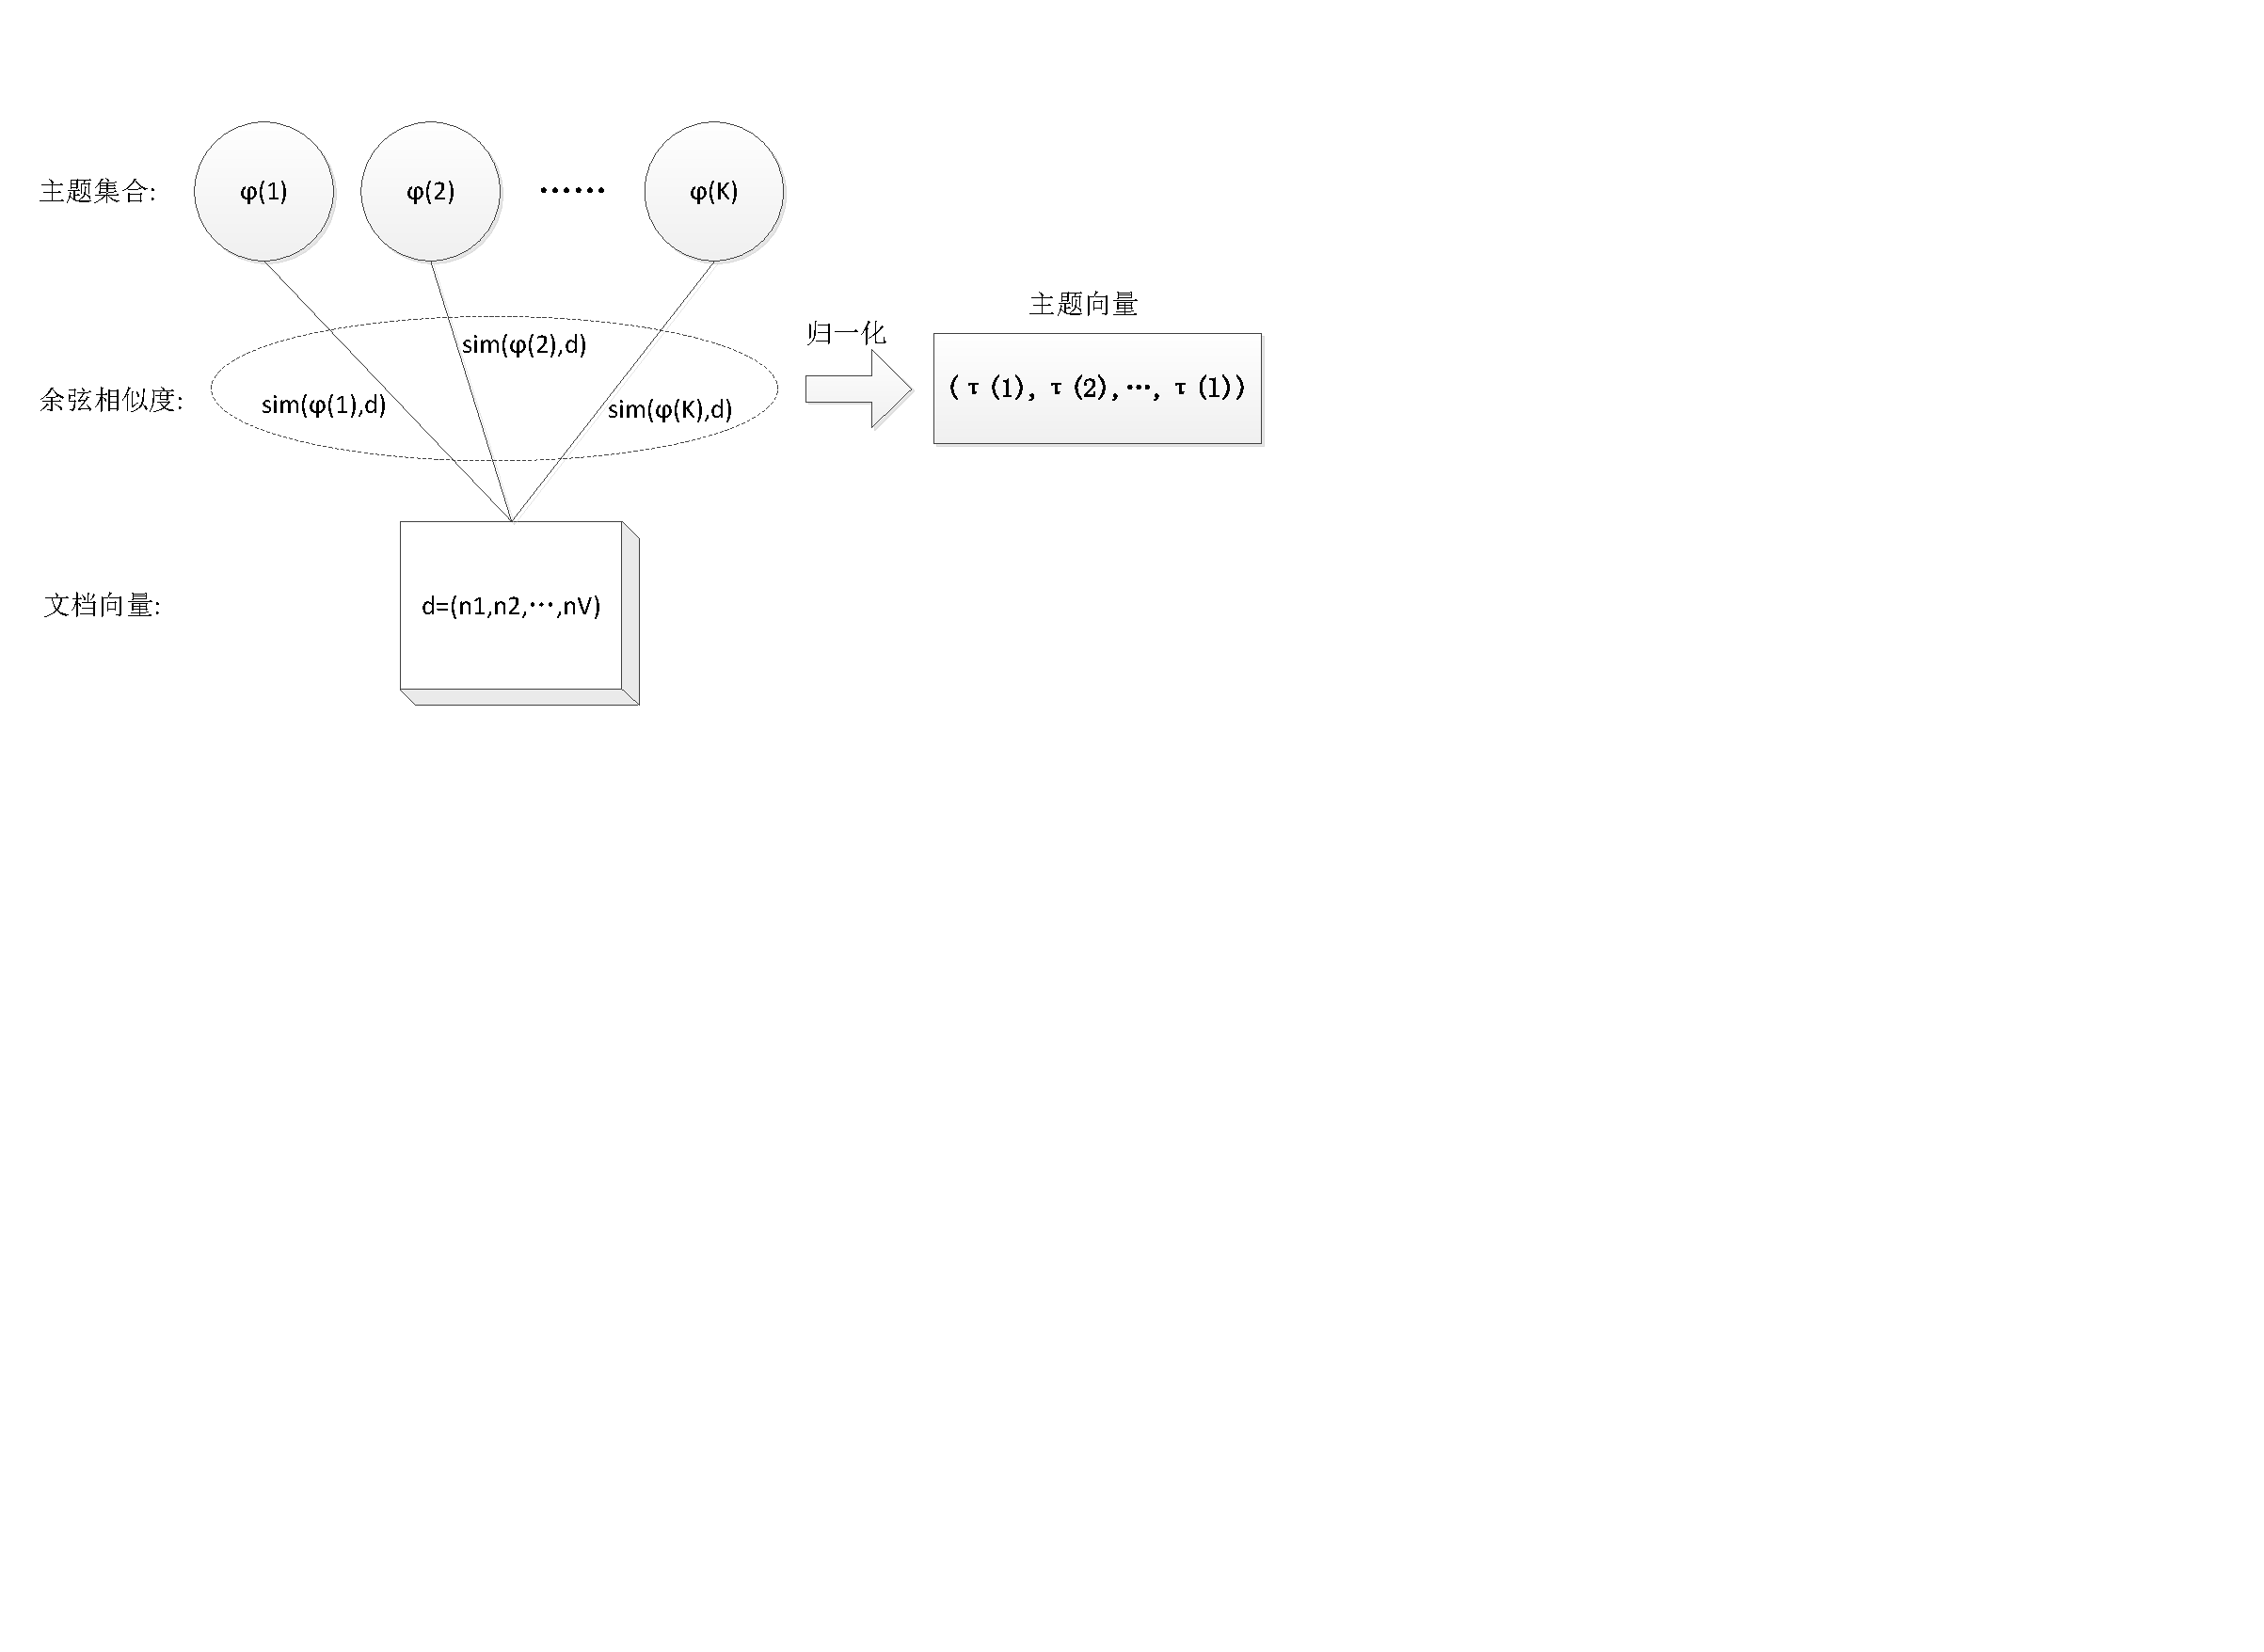
\includegraphics[width=\textwidth]{identifytopic.pdf}
\caption{基于相似度的长文本主题识别算法过程示例}
\label{fig:identifytopic}
\end{figure}

从图\ref{fig:identifytopic}中可以发现,主题集合中的$K$个主题分布$\vec{\phi_1},\vec{\phi_2},...,\vec{\phi_K}$在经过LDA推理后,其每个值得到的都是关于词汇表$V$中词汇的权重,从而组成一个$|V|$维的向量,这与文档向量$\vec{w}$的维数是一样的,当然这里的$\vec{w}=(n_1,n_2,...,n_{|V|})$,即对词汇表中每个词汇的频数(因为这里只有一篇文档,没有办法将文档向量表示成TF-IDF值)。然后通过计算主题分布于文档向量间的相似度$d_k=sim(\vec{\phi_k},\vec{w})$,得到一个新的$K$维向量,记为$\vec{s}=(d_1,d_2,...,d_K)$,但是这个向量中每个值之和并不为1,因此要进行一次归一化操作从而得到一个修正后的向量$\vec{s'}$:
\begin{equation}
  \vec{s'}=(d_1',d_2',...,d_K'),~~(d_k'=\frac{d_k}{\sum_{i=1}^{K}d_i},k\in[1,K])
\end{equation}
其中$d_k'$表示文档$d$拥有第$k$个主题的权重。然后,对$\vec{s'}$中的每个值进行从大到小的排序,排序后得到向量$\vec{s''}=(d_{k_1},d_{k_2},...,d_{k_K})$,其中$d_{k_i}$表示文档中编号为$k_i$的主题占有的权重,$i$表示该主题所占的权重在文档$d$中的重要性排在第$i$位。最后,对于给定的$\epsilon$,在$\vec{s''}$中选择前$l$个主题且满足$\sum_{i=1}^{l}d_{k_i}>\epsilon$。这时文档$d$的主题向量$\vec{\tau}$为:
\begin{equation}
  \vec{\tau}=(d_{k_1},d_{k_2},...,d_{k_l})~~(l\in[1,K])
\end{equation}

这个算法的时间复杂度是$O(K\cdot |V|)$,因为在计算主题分布和文档的相似度时,消耗的时间是$O(K\cdot |V|)$,在之后对向量权重进行排序的时候,平均时间复杂度达到$O(K\cdot log~K)$,很显然$log~K\ll|V|$,所以总共的时间复杂度是$O(K\cdot |V|)$。

\subsubsection{基于标签的主题分析技术}
对于上述提出的算法,可以基本实现对新文本进行主题标注的功能,但是上述算法存在一个很重要的问题,准确地说应该是主体模型LDA导致的一个问题。因为LDA是无监督学习,与K-mean等聚类算法相似,虽然它们可以计算出最后$K$个主题分布,但是对于每个主题分布的实际含义还需要人工标注,通过观察主题分布中的主题词来判断用什么词可以概括相应的主题。如表格\ref{tbl:topics}所示,第一行中的主题名称都是有人工标注的,这无疑造成了很大的麻烦,原因如下。
\begin{itemize}
  \item 自动化:在信息自主流动的机制中,由于主题数量巨大,主题也会不断地更新,因此用户不适合每次都使用手动标注,更好的办法是将更多的任务交给每个节点的智能系统进行处理。
  \item 歧义性:在表格中可以看到,虽然第一列标注为艺术,但是这一列的主题词也可以换成一个更加小的概念,比如电影艺术等等。同样第二列主题标注为财务,但是同样也可以认为是预算、经济等相同意义的词。
\end{itemize}

\begin{table}
\caption{主题模型训练后的主题示例}
\centering
\begin{tabular}{cccc} 
\hline
“艺术” & “财务” & “孩子” & “教育” \\
\hline
新的 & 百万 & 小伙伴 & 学校\\
电影 & 税收 & 女性 & 学生\\
展览 & 项目 & 人们 & 大学\\
音乐 & 上亿 & 多年 & 教育\\
影片 & 政府 & 家庭 & 教师\\
播放 & 每年 & 工作 & 高等\\
乐器 & 开销 & 家长 & 公开的\\
最好的 & 全新的 & 说 & 多媒体\\
演员 & 省市 & 回家 & 基础的\\
首次 & 计划 & 福利 & 试卷\\
戛纳 & 资金 & 爸爸 & 丰富的\\
剧院 & 扶植 & 比例 & 电子化\\
电影院 & 企业 & 关心 & 准时\\
爱 & 繁荣 & 生活 & 兴趣\\
票房 & 单位 & 愉快的 & 山区\\
\hline
\end{tabular}
\label{tbl:topics}
\end{table}

对于如今的互联网文本来说,文本资源其实不仅仅包含纯文本,而且还有一些元数据,其中最常见的新闻和博客资源中还包含了标签信息。因此,现在的问题是如何利用这些文本的标签的信息来重新训练主题,使得训练出来的主题都自动分配到一些标签。这里有两个问题,一个是如何通过语料库训练出带有标签的主题,另一个是如何给文档赋上多个带有标签的主题。对于第一个问题,一个比较成熟的方法是利用Labeled-LDA模型,或者L-LDA\cite{ramage2009labeled}重新训练这些主题。这里先对L-LDA模型进行简单的说明,进而对比该模型生成的主题与传统LDA生成的主题的不同之处,以及如何在下文中的进行修改使用。

L-LDA同样是一个概率图模型,其模拟了一个带有标签的文档集合的生成过程,换句话说,其充分利用了互联网上文档自带的标签数据。与LDA相同的地方是在生成过程中,每个单词依然是从一个选定的主题中生成的,但不同的是,该模型是一种有监督学习算法,通过分析标签与主题之间的对应关系来判断文档对应的标签是什么。接着上文的形式化定义,现在假设共有$K$个不同的标签对应$K$个不同的主题,


\subsection{短文本信息的挖掘与建模方法}

\subsection{关联性文本的挖掘与建模方法}

\subsection{文本流的挖掘与建模方法}

\subsection{小结}
